\section{Технический проект}
\subsection{Общая характеристика организации решения задачи}

Необходимо спроектировать и разработать сайт портфолио, который должен способствовать продвижению фотографа в социальных сетях и на рынке.

Интернет-сайт портфолио представляет собой набор взаимосвязанных электронных страниц, которые сгруппированы по разделам, содержащие текстовую, графическую информацию (изображения). Каждая страница web-сайта – это текстовый документ, написанный на языке программирования (HTML, CSS, JavaScript, Python).

\subsection{Обоснование выбора технологии проектирования}

В современном мире, где визуальное восприятие играет ключевую роль, создание веб-сайта для портфолио фотографа становится неотъемлемой частью представления своего творчества. Информационное пространство, насыщенное разнообразными программными решениями, предоставляет множество инструментов, способных подчеркнуть уникальность и профессионализм в области фотографии.

\subsubsection{Описание используемых технологий и языков программирования}

В процессе разработки web-сайта используются программные средства и языки программирования. Каждое программное средство и каждый язык программирования применяется для круга задач, при решении которых они необходимы.

\subsubsection{Язык программирования Python}

Python — это универсальный язык программирования, который также может использоваться для веб-разработки. Существует несколько фреймворков, таких как Django и Flask, которые позволяют разрабатывать веб-приложения на Python. Python обеспечивает чистый синтаксис, богатую стандартную библиотеку и поддержку объектно-ориентированного программирования, что делает его популярным выбором для веб-разработчиков.

\subsubsection{Язык программирования JavaScript}

\paragraph{Достоинства языка JavaScript}

JavaScript является языком программирования, который обеспечивает динамическое взаимодействие на веб-страницах. Он позволяет создавать интерактивные элементы, изменять содержимое страницы в реальном времени, выполнять асинхронные запросы к серверу и многое другое. JavaScript является одним из ключевых инструментов для создания современных, интерактивных веб-приложений.

\subsection{Диаграмма представлений и схема обмена данными между представлениями}

Диаграмма представлений описывает особенности физического представления разрабатываемой системы. Она позволяет определить архитектуру системы, установив зависимости между программными представлений, в роли которых может выступать как исходный, так и исполняемый код. Основными графическими элементами диаграммы представлений являются представления, интерфейсы, а также зависимости между ними. На рисунке \ref{comp:image} изображена диаграмма представлений для проектируемой системы. Она включает в себя сервер с операционной системой, на которой установлена система управления содержимым, включающая в себя базу данных и интерфейс. Помимо этого на диаграмме изображен клиентский компьютер с операционной системой, на которой установлен браузер.

\begin{figure}[ht]
	\center{\includegraphics[width=1\linewidth]{comp}}
	\caption{Диаграмма представлений}
	\label{comp:image}
\end{figure}

Любое представление должно быть вызвано в сценарии страницы web-сайта. Web-страница передает данные.

На рисунке \ref{data:image} представлена схема обмена данными между сценариями представления при вызове представления на странице сайта.


\begin{figure}[ht]
	\center{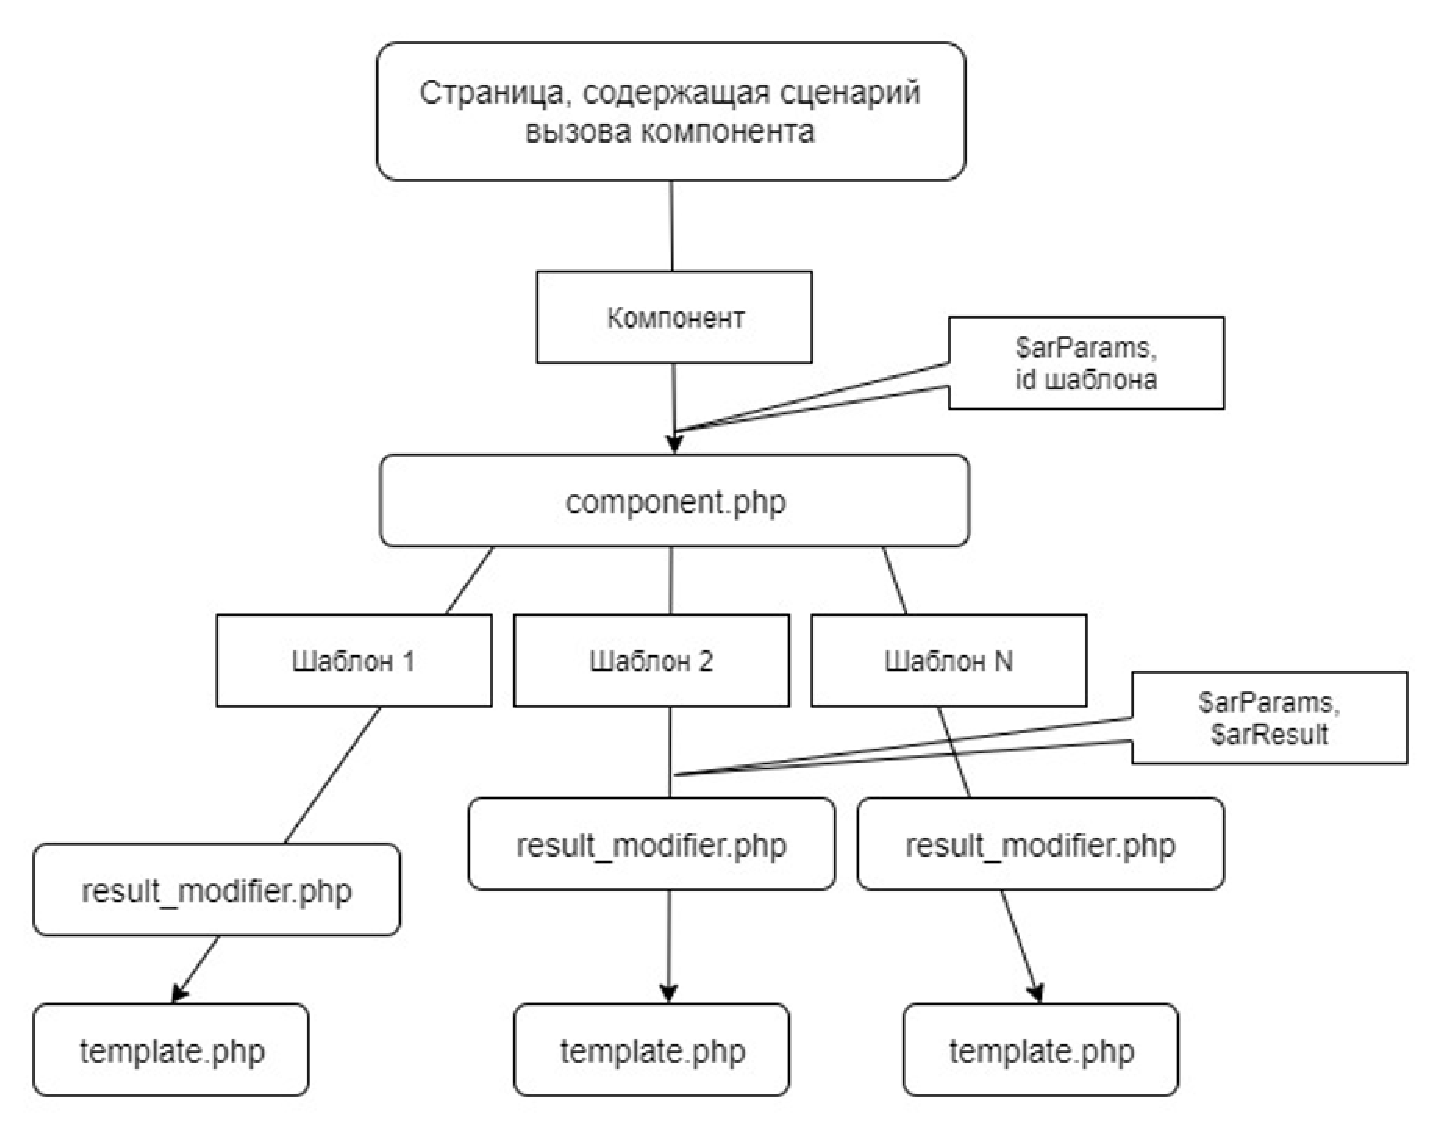
\includegraphics[width=1\linewidth]{data}}
	\caption{Диаграмма представлений}
	\label{data:image}
\end{figure}

В файле server.py написан код, который представляет собой простое веб-приложение на Python, использующее фреймворк WSGI (Web Server Gateway Interface).

Здесь импортируются различные библиотеки, классы и функции, которые используются в приложении, такие как CGI, Waitress для веб-сервера, различные представления (views) и функции для работы с файлами и базой данных. Словарь urls соотносит URL-пути с соответствующими представлениями. Когда приходит запрос, код использует этот словарь для определения, какой обработчик использовать для данного URL. Основная функция app обрабатывает POST запрос для загрузки файла, извлекает данные из формы, вставляет изображение в БД и возвращает ответ в формате JSON. Обработка GET запроса происходит с логики определения и вызова соответствующего представления и логики для обработки статических файлов, определение MIME-типа и кодировки для ответа, а также установка заголовков ответа и возврат данных в ответе.

\subsection{Диаграмма размещения}

Диаграмма размещения (рис. 3.2) отражает физические взаимосвязи между методами и представлениями.

\begin{figure}[ht]
	\center{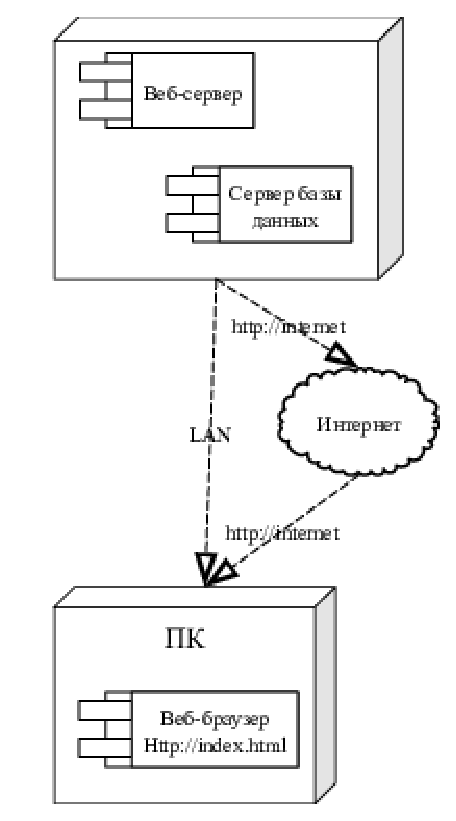
\includegraphics[width=0.57\linewidth]{place}}
	\caption{Диаграмма размещения}
	\label{place:image}
\end{figure}

Она является хорошим средством для показа маршрутов перемещения объектов и компонентов в распределенной системе.

\subsection{Содержание информационных блоков. Основные сущности}

Проанализировав требования, можно выделить две основных сущности:
\begin{itemize}
	\item "<Пользователь">;
	\item "<Добавление фотографии">;
\end{itemize}

В состав сущности "<Пользователь"> можно включить атрибуты, представленные в таблице 3.1.

\begin{xltabular}{\textwidth}{|l|l|p{1.7cm}|X|}
	\caption{Атрибуты сущности "<Пользователь">\label{news:table}}\\ \hline
	\centrow Поле & \centrow Тип & \centrow Обяза\-тельное & \centrow Описание \\ \hline
	\thead{1} & \thead{2} & \centrow 3 & \centrow 4 \\ \hline
	\endfirsthead
	\thead{1} & \thead{2} & \centrow 3 & \centrow 4 \\ \hline
	\finishhead
	id & ObjectId & true & Уникальный идентификатор \\ \hline 
	login & String & true & Логин \\ \hline 
	password & String & true & Пароль \\ \hline 
\end{xltabular}

В состав сущности "<Добавление фотографии"> можно включить атрибуты, представленные в таблице 3.2.

\begin{xltabular}{\textwidth}{|l|l|p{1.7cm}|X|}
	\caption{Атрибуты сущности "<Добавление фотографии">\label{news:table}}\\ \hline
	\centrow Поле & \centrow Тип & \centrow Обяза\-тельное & \centrow Описание \\ \hline
	\thead{1} & \thead{2} & \centrow 3 & \centrow 4 \\ \hline
	\endfirsthead
	\thead{1} & \thead{2} & \centrow 3 & \centrow 4 \\ \hline
	\finishhead
	id & ObjectId & true & Уникальный идентификатор \\ \hline 
	imagename & String & true & Название фото \\ \hline 
	imagedesc & String & true & Описание фото \\ \hline 
	imagecountry & String & true & Страна, где сделано фото \\ \hline 
	image & LONGBLOB & true & Фото \\ \hline 
\end{xltabular}
